\documentclass{lab}

\usepackage{graphicx}
\usepackage{float}

\title{ENGG1003 - Lab 1}
\author{Brenton Schulz}
\date{\today}

\begin{document}
\maketitle

\section{Introduction}
This laboratory exposes you to the fundamental tools required to write computer programs in C. No prior programming experience is assumed but if you don't have basic computer literacy you're gonna have a bad time.

\section{C Programming Basics}
In order to write programs in C (and most other languages) the following software tools are required:

\begin{itemize}
\item An \textit{editor}, to create and edit raw text files.
\item A \textit{compiler}, to convert your text files into an \textit{executable} file.
\end{itemize}

A programming editor is very different to a \textit{word processor} (eg: Microsoft Word) in that it displays and stores raw ASCII text only. What you see printed to the screen represents the \textit{actual data} stored in the file. By contrast, Word will store a combination of text and display formatting and, as such, is not suitable for writing code.

Programming editors will generally have features optimised for coding, such as:

\begin{itemize}
\item Syntax highlighting
\item Line numbering
\item Auto completion
\item Pre-emptive error notifications
\item Communication with the compiler to highlight errors
\item Automatic indenting
\item Highlighting of matching blocks 
	\begin{itemize}
		\item ie: an easy method to find matching pairs of ( ), \{ \}, " ", etc.
	\end{itemize}
\end{itemize}

It is hoped that you will discover these features and learn to work with them. In time you will learn which features work well with your style and which simply get in the way.

For the time being the ``compiler'' noun will be used to colloquially reference a highly complex set of software tools which turn your source code into an executable binary file. You will be shielded from the details until otherwise necessary.

\subsection{Introduction to OnlineGDB}

OnlineGDB is a basic (\textit{very} basic) browser-based development environment for a variety of programming languages. It gives you access to an editor, a small amount of cloud storage, compiler, and standard input~/~output. It also contains a \textit{debugging} feature however for technical reasons\footnote{It only allows one debug session per IP address. The entire campus uses the same public IP so we can't use it in labs.} we won't be using it.

All compilation and execution is performed on the OnlineGDB server. As such, the service has an incredibly low barrier to entry: there is (almost) zero installation/configuration required to get started running code.

\textbf{Task:} Open a web browser and navigate to \url{http://www.onlinegdb.com}.\\ \\ \textbf{NB:} If a demonstrator sees you using Edge or IE they may instinctively think you need more help than students using Chrome or Firefox.

\begin{figure}[H]
\begin{center}
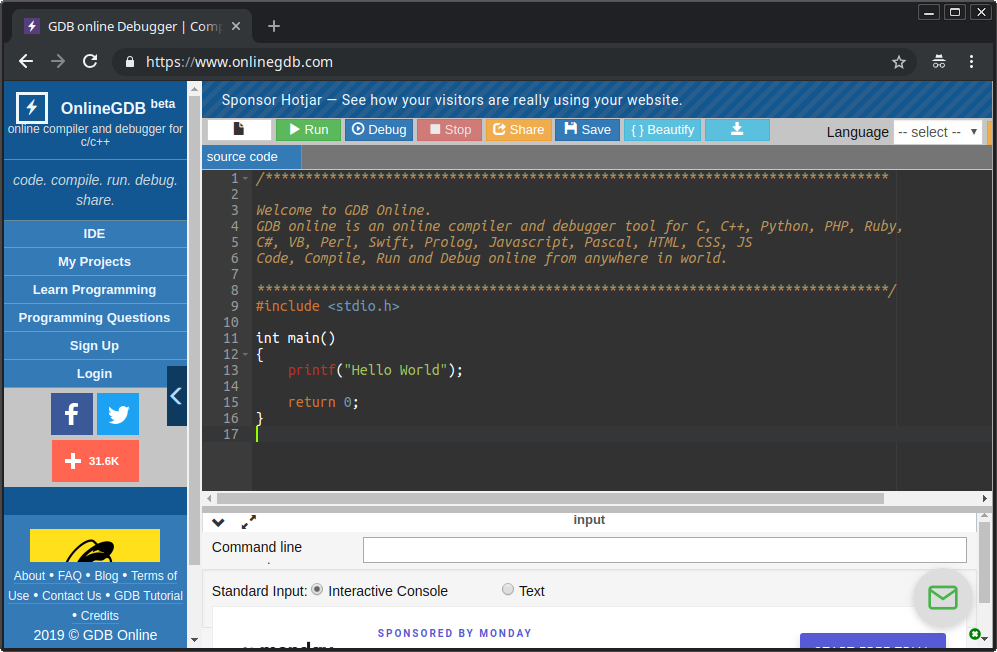
\includegraphics[width=\textwidth]{onlinegdb.png}
\end{center}
\caption{The view when OnlineGDB is first opened.}\label{fig:onlinegdb}
\end{figure}

After OnlineGDB has loaded you will be greeted with the screen seen in Figure \ref{fig:onlinegdb}. The large area in the middle is the editor screen, this is where you will type C code. Immediately you can observe that this editor supports line numbering and syntax highlighting.

Above the editor is a toolbar which, from left to right, performs the following functions:

\begin{enumerate}
\item Create a blank new file
\item Run the project
\item Debug the project (not used in ENGG1003)
\item Stop execution of a running program
\item Share - Generates a link to your current source code
\item Save - When logged in this saves the project files to your personal cloud storage
\item \{ \} Beautify - Modifies your code's whitespace to adhere to the OnlineGDB indenting style (NB: I tried this at time of writing and it didn't work on my personal computer. Go figure.)
\item Download - Downloads the currently viewed file.
\end{enumerate}

The area below the editor is where standard output is written to and standard input read from. When the code is run its appearance changes to that of a basic console (ie: the GUI elements disappear and it becomes just text).

\textbf{Task:} Configure OnlineGDB to run C code by selecting ``C'' from the ``Language'' drop-down box in the upper-right. This website supports many languages\footnote{MATLAB is not one of them because it is a \textit{very} expensive commercial package} so feel free to come back here later if you're interested in learning any of the others. Python, although not taught in an Engineering degree, is a common choice for Engineering PhD students as a free MATLAB alternative and is probably worth playing around with.

\textbf{Task:} Click the green Run button. The box at the bottom of the screen will produce a ``Compiling'' animation and, after execution of the template code, will produce the output seen in Figure \ref{fig:onlinegdb_hello}.

\begin{figure}[H]
\begin{center}
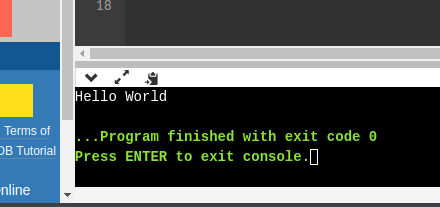
\includegraphics[width=0.7\textwidth]{onlinegdb_hello.png}
\end{center}
\caption{A cropped screenshot showing the "Hello World" program output.}\label{fig:onlinegdb_hello}
\end{figure}

\textbf{Off-topic note:} Remember the ``returns zero to the operating system'' comment in lecture 1? Well that's what the text ``...Program finished with exit code 0'' is referencing. The 0 is the number that \texttt{main()} \textit{returned}. We will learn about \textit{function return values} later in the semester.

\textbf{Tasks:} 

\begin{enumerate}

\item Running the default template demonstrates \textit{standard output}, modify the code to match that in Listing~\ref{lst:stdio}. While making the changes you will observe OnlineGDB's auto-complete features. When, for example, you type a double quote " character it \textit{automatically} types two and places the cursor between them. It will also provide auto-complete suggestions, although many of them will be inappropriate (it is, after all, just a computer program; not a science fiction grade artificial intelligence).

What other ``helpful'' editor behaviour did you notice? Some of it will be annoying at first (some of it will be annoying \textit{forever}) but learning to work with the editor's features will improve your coding speed in the long term.

\begin{lstlisting}[style=CStyle,caption=A basic C program which demonstrates input and output.,label=lst:stdio]
#include <stdio.h>

int main() {
	int k;
	scanf("%d", &k);
	printf("You entered: %d\n", k);
	return 0;
}
\end{lstlisting}

\item After editing the code press Run. After it is compiled you will notice that the console is just displaying a cursor. This is because \texttt{scanf()} waits for data to be typed (specifically, it will wait until a new line character, ASCII value 10, is sent).

\item Type an integer and press \texttt{enter / return}. There will be some ``lag'' because the data is being sent to OnlineGDB's server before being displayed.

\item After pressing enter the console should display the text ``\texttt{You typed: 123}''.

\item Run the program again except this time don't type just an integer, try typing a word, or a word containing a number, or a number followed by letters (with and without a space). What is the behaviour each time? Are you getting annoyed by the slow compile time and lag yet? OnlineGDB may be simple but it is, at times, a compromise.

\end{enumerate}


\pagebreak
\section{Compiler Errors and Warnings}

This section will demonstrate several common compiler \textit{errors} and \textit{warnings}.

An error occurs when the code does not meet the rigorous and unambiguous syntax rules specified in the ANSI C standard and, as such, the compiler does not know how to interpret the code. For example, if you miss a " symbol inside a \texttt{printf()} where does the text to be printed end? This can't be assumed because there are not enough rules about what you can and can't write in this context. As such, missing a " will produce a \textit{syntax error}.

By contrast, a warning occurs when the code is in some way ``mildly'' problematic but the compiler is still able to make assumptions about what the code should do and produce a binary executable. For example, if the \texttt{return 0;} at the end of \texttt{main()} is missing the compiler will throw it in for you because, well, what else is it going to do at the end of \texttt{main()}?\footnote{The programmer could want \texttt{main()} to return a value other than zero but it is overwhelmingly common to just return zero here. Historically, a program returning zero means ``the program finished without error'' and non-zero indicates some kind of error code.}

Unfortunately compiler errors can be \textit{highly} technical and difficult to interpret. Furthermore, they often report an error on a line \textit{after} the actual mistake! The exercises below will give you some experience with interpreting compiler errors but this is a topic in which you will likely engage in ``life-long learning''.

\subsection{Missing a semicolon}

\textbf{Task:}
\begin{enumerate}
	\item If you have not done so already, get the code shown in Listing \ref{lst:stdio} working correctly.
	\item Remove the semicolon (the ; character) from the end of line 4.
	\item Compile the code, what error did the compiler produce? Which line does it say the error is on?
	
	The compiler errors will look something like Listing \ref{lst:errs}.
	
	\begin{lstlisting}[caption=The multiple errors produced by removing a \textit{single} semicolon.,label=lst:errs,basicstyle=\ttfamily,frame=single]
main.c: In function ‘main’:
main.c:14:5: error: expected `=`, `,`, `;`, `asm` or `__attribute__`
	before `scanf`
     scanf("%d", &k);
     ^
main.c:14:18: error: ‘k’ undeclared (first use in this function)
     scanf("%d", &k);
                  ^
main.c:14:18: note: each undeclared identifier is reported only once for
	each function it appears in
	\end{lstlisting}
\end{enumerate}
	
Lets break this down a bit. Each error starts with a location, the syntax is: \texttt{{file}:{line}:{column}}. So \texttt{main.c:14:5} means the file \texttt{main.c} at line 14, column\footnote{\textit{Column} means the number of characters since the start of the line} 5.

The first error (\texttt{error: expected '=' , ‘,’, ‘;’, ‘asm'}... etc.) is telling you that something was missing and the compiler noticed the omission at line 14. In this case we removed a ; so that's what is missing. Note, however, that while the error was reported to be on like 14 the omission was actually on line 13! Also observe the extra technical jargon that you don't understand yet (what is \textit{\_\_attribute\_\_}??). Some of these are, in fact, beyond the scope of ENGG1003, you have to get used to reading text you don't understand and extracting the small pieces of information you actually need.

Let's look at the second error: \texttt{'k' undeclared}. Wait, wasn't \texttt{int k} still in our source code? Why is the compiler complaining that it is undeclared when it is \textit{right there}? The problem is that by removing the semicolon the declaration syntax was incorrect, so the compiler did not interpret that line as a declaration. It didn't find the expected ; threw its hand in the air and gave up.

The final line (\texttt{each undeclared identifier...} etc.) is just telling you that if you forget to declare a variable the compiler will only tell you about it \textit{once}. This is because it could appear multiple times and producing the same error over and over is redundant and confusing.

Lets try a different syntax error.

\subsection{Missing a Quote Symbol}

\textbf{Task:} Remove the closing " from the \texttt{printf} line so it reads:

\begin{lstlisting}[style=CStyle]
printf("You entered: %d\n, k);
\end{lstlisting}

You will see an immediate change to the syntax highlighting; all characters between where the " was and the end of the line are now green, as if they were still inside the double quotes. Take-home message: \textit{pay attention to syntax highlighting!}

Again, removing a \textit{single character} generated a slew of errors:

\begin{lstlisting}[basicstyle=\ttfamily]
main.c: In function ‘main’:
main.c:15:12: warning: missing terminating " character
     printf("You entered: %d\n, k);
            ^
main.c:15:5: error: missing terminating " character
     printf("You entered: %d\n, k);
     ^
main.c:16:5: error: expected expression before ‘return’
     return 0;
     ^
main.c:17:1: error: expected ‘;’ before ‘}’ token
 }
 ^
\end{lstlisting}

Observe how missing the closing " generates both and error and a warning at different locations. Why does it do this? To be honest, this is beyond my experience; I've only been using gcc for 20 years, there's always \textit{something} that you haven't learned yet. In the end it doesn't matter, an error exists that needs to be fixed before the compiler can output an executable.

Missing the " generated two other errors. By missing the " the \texttt{printf} \textit{expression} was not completed. In C an expression can be thought of as "a complete line of code that does something unambiguous". This is a \textit{very} informal definition but it will do for now. In order to complete the \texttt{printf} expression the syntax rules require the closing ", a closing right parenthesis ) [to match the opening left parenthesis (] and a semicolon ;. Removing the " character makes the compiler think that the existing ``\texttt{);}'' string at the end of the line is actually part of the data to be printed, not part of the C expression syntax (as such, the expression was never finished, leaving the compiler with an unresolved tension that will stay with it \textit{all day}\footnote{\url{https://xkcd.com/859/}}.

Remember how missing a ; caused errors on lines \textit{below} where the error actually was? Well the same thing has happened here. Because the \texttt{printf()} line was malformed an error occurred on the line below it (\texttt{expected expression before return}) \textit{and} the one below that (\texttt{expected ; before \} token}); and you thought your \textit{ex} was highly strung!

\pagebreak

\subsection{Failing to Define \texttt{main()}'s Return Type}

Enough about errors, the final example in this section demonstrates a compiler \textit{warning}. Unfortunately, OnlineGDB doesn't display the compiler output if only warnings are generated. If you are running \texttt{gcc} in Linux (as described at the end of this lab document) you won't have this problem\footnote{Yeah, I'm very biased towards Linux. It gets a bad rap because games, Microsoft Office, Adobe, and Autodesk don't support it but it is otherwise \textit{overwhelmingly} dominant. It runs: mobile phones (Android is a Linux derivative, iOS is a Unix variant), servers, supercomputers, ``internet of things'' devices, etc. As engineers you will probably see it in many places throughout your career, just hidden from the end user.}.

\textbf{Task:} Remove \texttt{int} before \texttt{main} and the semicolon in \texttt{return 0}, as per Listing \ref{lst:warn}

\begin{lstlisting}[style=CStyle,caption=Example code which generates a warning.,label=lst:warn]
main()
{
    int k;
    scanf("%d", &k);
    printf("You entered: %d\n", k);
    return 0
}
\end{lstlisting}

Attempting to compile this code generates the following compiler output:

\begin{lstlisting}[basicstyle=\ttfamily]
main.c:11:1: warning: return type defaults to ‘int’ [-Wimplicit-int]
 main()
 ^
main.c: In function ‘main’:
main.c:17:1: error: expected ‘;’ before ‘}’ token
 }
 ^
\end{lstlisting}

The error can be ignored here, lets focus on \texttt{warning: return type defaults to `int`}. The keyword which goes before \texttt{main()} specifies its \textit{return type}. This is the type of data which it sends back to the operating system on program exit, we will study function return types in later weeks. To my knowledge, operating systems only support the \texttt{int} return type (ie: an integer) so if you leave it out the compiler can quite safely \textit{assume} that's what should be there and only issue a warning instead of an error.

Generally speaking, warnings should be fixed when you see them. With experience you will know when they \textit{need} to be fixed (because the compiler is assuming something incorrectly) and when they can be ignored (because you have more important stuff to fix first).

No doubt you will see \textit{many} other errors and warnings during your foray into C programming. I still occasionally see new ones! If in doubt, throw the compiler output into Google, chances are someone on Stack Overflow\footnote{Why are you even taking this course? Stack Overflow is all you \textit{really} need, right?} has written a good explanation about it.

\pagebreak
\section{Comments}

So far all the code examples have been very basic and (hopefully) easy enough to read. In ``real'' projects, however, this is rarely the case and the code needs some kind of explanation for the reader to quickly, and accurately, understand what it does\footnote{Despite what you might believe experienced engineers and programmers are not wizards, our understanding is not \textit{magic}, it is based on experience and frequently needs supplementing with code comments.}.

You will hopefully gain experience with code comments as you progress through this course (and the rest of you career!) but for now we will just see the basics. Any text in the source files\footnote{Did I forget to define what source code, or source files, are? It is just another word for any programming code. It can also be called a source \textit{listing}.} which:

\begin{itemize}
\item Is between \texttt{/*} and \texttt{*/}, or
\item Is between \texttt{//} and the end of the line
\end{itemize}

is \textit{totally ignored} by the compiler and called a ``comment''.

Code comments are a place for you to explain how your code works, or what it does, to future people who work with it. It is also a great place to leave little memos to yourself, typically in the form of:

\texttt{// TODO: Fix this because <reasons>}.

In fact some code editors (like the Linux editor \texttt{vim}) will automatically highlight the text \texttt{TODO} so it is easy to find.

\textbf{Task:} Take whatever source code is currently shown in OnlineGDB and add some comments in various places. Compile the code and observe that they have no effect.

Students frequently ask what should and should not be commented. In this course your comments should be written such that a student who is on track to achieve 50\% can understand what your code does without having to consult external reference material. This will seem overly verbose but it will be used in lieu of a better standard. As a general rule: if you needed to look up something in a reference manual when writing the code write a comment explaining it. For example:

\begin{lstlisting}[style=CStyle]
printf("%d\n", x); // %d formats an integer
\end{lstlisting}

Anything which, at first glance, appears to be at least a little bit cryptic should probably get a comment.

\pagebreak
\subsection{Intrinsic Documentation}

As a supplement to comments, \textit{intrinsic documentation} is the idea behind choosing informative names for variables and functions\footnote{No, you don't need to know what a function is yet. It is in week 5 or so.}. Compare, for example, the following two code listings:

\begin{lstlisting}[style=CStyle]
int main()
{
	float x, y;
	scanf("%f", &x);
	y = x*9.0/5.0 + 32.0;
	printf("%f\n", y);
}
\end{lstlisting}

\begin{lstlisting}[style=CStyle]
int main()
{
	float tempFahrenheit, tempCelcius;
	scanf("%f", &tempCelcius);
	tempFahrenheit = tempCelcius*9.0/5.0 + 32.0;
	printf("%f\n", tempFahrenheit);
}
\end{lstlisting}

The first one, especially without comments, is cryptic and not possible to understand without more information. The second, even if you don't understand all the code, quite intuitively converts Celcius to Fahrenheit.

You will observe that my notes break intrinsic documentation rules all the time. Sorry about that (the examples in notes will also tend to not do anything particularly useful, so it gets difficult when you want to document ``nothing'').

\pagebreak
\section{Basic Arithmetic in C}

So, it is Page \thepage{} of these notes and we haven't done anything \textit{useful} yet! Ok \textit{fine}, lets do some data processing.

In this section we will do some basic arithmetic on numbers which are read from the console (ie: read from \texttt{stdin}). Since we haven't learnt much C (or even much programming in general) these examples are either going to be a bit boring (because they don't do much) or look like black magic (because you haven't learned how they work yet). I have to ask you just to go through the motions at this stage, hopefully exposure to the code below now will make it easier to understand how it works in the coming weeks.

Lets start with the basic C arithmetic operators:

\begin{table}[H]
\centering
\begin{tabular}{|l|c|}
\hline
Operation      & C Symbol \\
\hline
Addition       & +        \\
Subtraction    & -        \\
Multiplication & *        \\
Division       & /       \\
\hline
\end{tabular}
\caption{Basic arithmetic operators in C}
\end{table}

These are all \textit{binary} operators, meaning they operate on two \textit{operands}\footnote{An operand is one of the ``things'' that a mathematical operator operates on. Eg: In a + b the variables a and b are operands.}. This may feel obvious, but C includes several \textit{unary} operators and even a \textit{ternary} one (that nobody uses because it's confusing). Each operand could be a variable (eg: \texttt{a + b}), a constant (eg: \texttt{a + 5}) or some complicated expression (eg: \texttt{(2*a + 6) / (12 + b - x)} )\footnote{I contemplated leaving this closing parenthesis out to give you unresolved tension but I'm not quite \textit{that} evil.}.

We begin with a basic example:

Modify your code to match that of Listing \ref{lst:arithmetic1}.

\begin{lstlisting}[style=CStyle,caption=A basic arithmetic example,label=lst:arithmetic1]
#include <stdio.h>

int main() {
	int k;
	printf("Enter an integer: ");
	scanf("%d", &k);
	k = 2*k;
	printf("That integer doubled is: %d\n", k);
	return 0;
}
\end{lstlisting}

Notice that this code has a \textit{slightly} improved user experience to previous examples; it produces a prompt (\texttt{Enter an integer: }) which tells you what to do. Also notice that the first \texttt{printf()} does \textit{not} end with a \texttt{\textbackslash n} (newline), so the number you type appears on the same line as the prompt.

The line \texttt{k = 2*k} takes the value of \texttt{k}, multiplies it by 2, then assigns that result back into the variable \texttt{k}. This is a \textit{crucial} concept in programming: the \texttt{=} symbol is \textbf{not} equality, \texttt{k = 2*k} is \textbf{not} an equation, it is \textit{assignment}. Assignment takes what's on the right, evaluates it, then stores it into the variable on the left.

\subsection{Operator Precedence Basics}

Just like in ``normal'' algebra different operators take precedence over others (PEMDAS / BODMAS anyone? How about those Facebook posts where \textit{everybody} gets this wrong?). You can view the full C operator precedence here: \url{https://en.cppreference.com/w/c/language/operator_precedence} but you don't need to learn all of it now, it will be covered more in future lectures.

For now we will observe some basic examples and look at how engineers can deal with the complexity of full C operator precedence.

The predominant engineer's approach to this topic is to vaguely learn how the language behaves and then throw parentheses everywhere just to be \textit{absolutely sure} that the intention is not ambiguous. In the end it is \textit{other people} who will have trouble reading your code, not the compiler, so you might as well make their job easy.

\textbf{Task:} Implement the following equation in C:

\begin{equation}\label{eq:fraction}
y = 2x+3\times5
\end{equation}

using the template in Listing \ref{lst:arithmetic2}.

\begin{lstlisting}[style=CStyle,caption=A basic arithmetic example,label=lst:arithmetic2]
#include <stdio.h>

int main() {
	float x;
	float y;
	printf("Enter a number: ");
	scanf("%f", &x); // Note change of %d to %f
	// y = ??? uncomment this line and write your answer instead
	printf("y: %f\n", y);
	return 0;
}
\end{lstlisting}

You will notice a few new things about Listing \ref{lst:arithmetic2}. Firstly, it uses the \texttt{float} datatype. This type will store any real number with a magnitude of $1.2 \times 10^{-38}$ to $3.4 \times 10^{38}$ with a precision of approximately 6 decimal digits. Its bigger brother, the \texttt{double} will be seen later.

The other major change is that inside \texttt{scanf} and \texttt{printf} the \texttt{\%d} has changed to \texttt{\%f}. The \texttt{f} stands for floating point, which is a standard method\footnote{The other major standard is known as \textit{fixed point}. Details are beyond ELEC1003 but you'll probably see it if you study enough digital signal processing (DSP).} for storing fractional numbers using only binary integers. The details are beyond this course, but you can read the details on Wikipedia: \url{https://en.wikipedia.org/wiki/IEEE_754}.

Back to the task at hand, have a go at implementing Equation \ref{eq:fraction} and see if the result works. Observe that you don't need to force precedence with parentheses because, in C, the multiplication operations are performed before addition.

As practice, implement the following equations (what happens when you choose x to force a division by zero?):


\begin{enumerate}
\item $y = \frac{9}{5} x + 32$
\item $y = \frac{x}{1 - x}$.  This one will require parentheses.
\item $y = x^2 + 2x$. \textbf{NB:} C does \textit{not} include an exponent operator. Implement $x^2$ as \texttt{x*x}:
\item $y = \frac{x + 2}{x - 1}$
\end{enumerate}

\pagebreak
\section{A Very Brief Introduction to Git}

\textit{NB: Git is not in the course outline so it isn't strictly required nor assessed. It is, however, incredibly useful and included here because several 3rd and 4th year course coordinators (and industry contacts) asked me to expose you to it. I agreed.}

Programming projects typically involve two potentially problematic issues:

\begin{enumerate}
	\item Multiple people contribute to the same project
	\item Programmers frequency want to ``roll-back'' to an earlier code version.
\end{enumerate}

The second item arises from the fact that after going down a problematic design pathway it is typically much faster to scrap the idea and start again than it is to try and fix all the problems you just created. The fastest way to do \textit{this} is to load up known-working code from the past and go from there.

As such, programmers designed so-called \textit{versioning} subsystems. These are ways of storing data which allows someone to access either a current or past version.

In this course it will be \textit{recommended} that you take advantage of the modern versioning system known as Git. It was developed for tracking code in the Linux kernel and has since expanded to be an industry standard; even Microsoft purchased the website GitHub because it was \textit{just better} than anything else they had developed internally. I am using Git for tracking changes while writing course content. The Git host GitHub is also doubling as cloud storage as I move writing between three different computers.

\textbf{Task:} Navigate to \url{https://github.com/bschulznewy/engg1003/blob/master/Lectures/Wk1/Friday/LectureFriWk1.pdf}, this is the GitHub ``repository'' that I have been using when writing ENGG1003 content. In particular, it is the lecture notes for the Friday Week 1 Lecture (I'm subtly trying to get you to read them ahead of time, apologies for improving your study efficiency).

The link is for a PDF document and you will see that GitHub automatically renders it inside the website. It will attempt to display any file directly linked to.

But that's not what we're here for, I want to show you the real power of Git: version tracking. Click on the ``History'' button to the top right of the PDF preview. You will be greeted with a view similar to that shown in Figure \ref{fig:githistory}. It lists the git \textit{commits} made which effect that file. A commit is a snapshot of what the entire repository looked like at a particular point in time. Each commit happens manually (ie: I type a command to cause a commit to be created) and is attached to a ``commit message'' which (hopefully) describes the changes which were made.

\begin{figure}[H]
\begin{center}
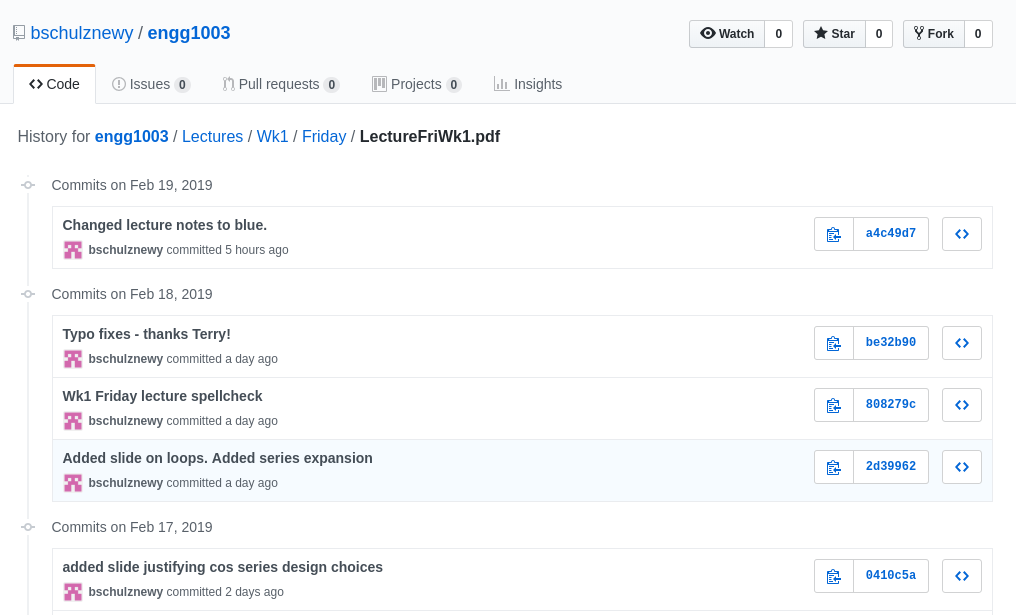
\includegraphics[width=0.8\textwidth]{github_lecture.png}
\end{center}
\caption{The git repo history for the Friday lecture notes.}\label{fig:githistory}
\end{figure}

Click on the top one (specifically the text ``Changed lecture notes to blue.'') and you will see what changed in this particular git commit.

\begin{figure}[H]
\begin{center}
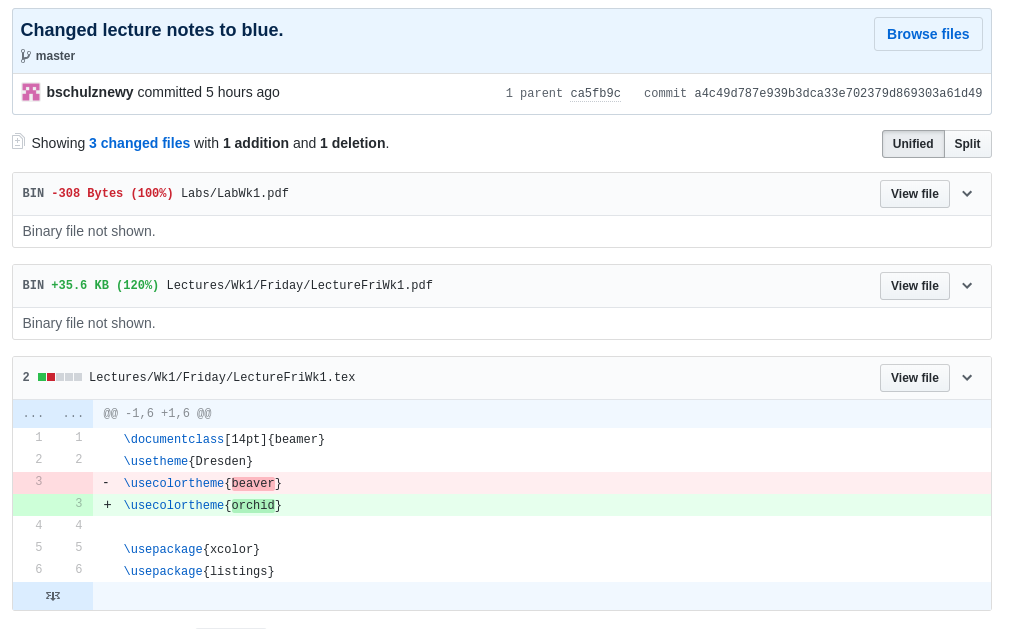
\includegraphics[width=0.9\textwidth]{github_lecture_changes.png}
\end{center}
\caption{The changes which occured in a particular commit.}\label{fig:gitchanges}
\end{figure}

The box at the bottom of Figure \ref{fig:gitchanges} shows the actual changes which occurred. In this case I changed the colour theme for the lecture notes to roughly match that of the first lecture. The changes to the PDF are not shown because they would be unintelligible garbage (it is a binary file, not text).

Click the ``View file'' button next to LectureFriWk1.pdf to view what the PDF looked like in this commit.

Browse through the other commits and observe the writing process for the Lecture 1 PDF, feel free to also browse the other files in the repository.

\textbf{Task:} Go to \url{www.github.com} and create a GitHub account. You will use it in later weeks when we swap to a development environment which supports Git. You can also use a GitHub account to login to OnlineGDB, allowing you to have your source files stored on their server.

\textbf{Task:} Read more about how Git works and what it does here: \url{https://developer.ibm.com/tutorials/d-learn-workings-git/}. You probably won't understand everything, but that's not important right now. Just get some general exposure to the ideas and we'll fill in the practicalities later.

\pagebreak
\section{Getting started with C in Ubuntu Linux - Optional}

Linux is not supported by university IT but, personally, I find it to be a fantastic development platform. The following instructions are completely optional, only do this if you are keen to learn.

Installing Ubuntu is beyond the scope of this document (and course). If you think this is a daunting task I would recommend only using the officially supported tools to complete ENGG1003. There are many thousands of websites and YouTube videos which will guide you through the Ubuntu (or Mint, Arch, etc.) installation process. \textbf{NB:} Installing a new operating system can \textit{very easily} destroy all existing software on a machine. Don't do this if you don't know what you're doing.

That out of the way, here's how you can get started. These steps assume a fresh Ubuntu 18.04 installation, in other distributions YMMV\footnote{Your mileage may vary. ie: this step might not work.}:

\begin{enumerate}
\item The C compiler in Linux (and OnlineGDB, and \textit{many} other platforms) is gcc (the GNU C Compiler). To install it, open a terminal (\texttt{ctrl + alt + t}) and type:

\texttt{\$ sudo apt install gcc libc6-dev gedit}\\ (the \$ indicates the terminal prompt, don't type that character)

When prompted, enter your password, wait a few seconds, press \texttt{enter} if it wants installation confirmation, and wait a few more seconds. An Internet connection is required for apt to download the required software.

The \texttt{libc6-dev} package provides all the basic C libraries (\texttt{printf} etc.) and \texttt{gedit} is a basic text editor.

\item Lets make a new directory for writing C files, type:
\begin{enumerate}
	\item \texttt{\$ mkdir c}
	\item \texttt{\$ cd c}
\end{enumerate}
The first command creates a directory called ``c'' and the second ``changes into'' that directory.

\item Create a new .c file. We will do this in \texttt{gedit} (because it is easy and simple) but there are many others (the more nerdy among you may want to learn \texttt{vim} or \texttt{emacs}. They are \textit{very} powerful editors).

Type: \texttt{\$ nohup gedit test.c \&} \\ (The \& symbol at the end of a command runs the command ``in the background''. This gives you the command line back straight away, instead of having to quit gedit first. Preceding the command with \texttt{nohup} stops \texttt{gedit} from closing if you close the terminal window)

\item Type out the code seen in Figure \ref{fig:gedit}.

\item Click the Save button (or type \texttt{ctrl + s}).

\begin{figure}[H]
\begin{center}
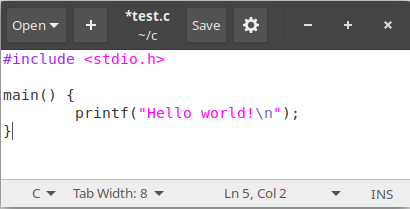
\includegraphics[width=0.5\textwidth]{gedit.png}
\end{center}
\caption{The gedit window with some C code typed out.}\label{fig:gedit}
\end{figure}

\item Move the \textit{keyboard focus} back to the terminal (ie: click the terminal window).

\item If you can see the command prompt yet, press \texttt{enter}

\item You can type \texttt{ls} to see a list of all files in the current directory. \texttt{test.c} should be there.

\item To compile the \texttt{.c} file run: \texttt{\$ gcc test.c -o test}

This will create a binary executable called \texttt{test}. If the \texttt{-o} \textit{command line argument} is not given \texttt{gcc} the binary file defaults to the name \texttt{a.out}.

\item Run \texttt{test} by typing: \texttt{\$ ./test}

The \texttt{./} is a special character string meaning ``relative to the current directory''. If you try to run \texttt{test} from any other directory nothing will happen because \texttt{test} is a built-in command. With most other names you will get a ``Command not found...'' error.

\item When the program runs you should see something similar to Figure \ref{fig:c_ubuntu}.

\item Go back to \texttt{gedit} and keep coding as you desire. Return to the command line to run \texttt{gcc} to re-compile your code. \textbf{NB:} The command line has a \textit{history} feature, pressing the up arrow will scroll through past commands, \textit{you don't need to type them out from scratch}.

\item If you enjoyed this you're a bit weird, welcome to the club! Recommended further reading would be a tutorial on \texttt{make} followed by investigations into more powerful editors like \texttt{vim}.

\begin{figure}[H]
\begin{center}
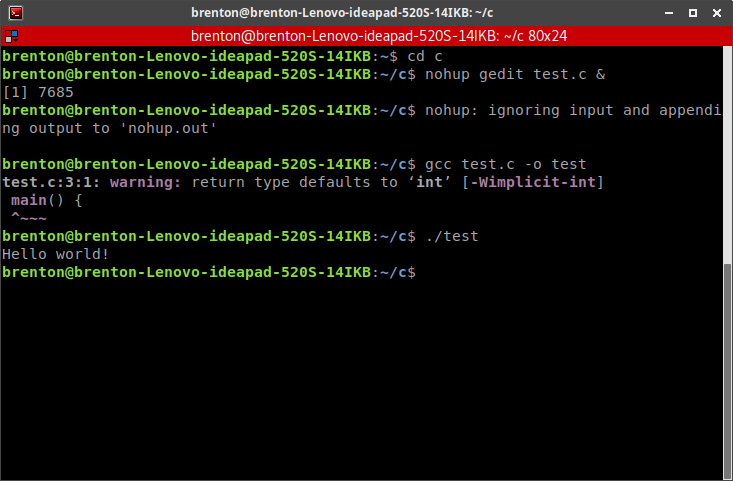
\includegraphics[width=0.8\textwidth]{c_ubuntu.png}
\end{center}
\caption{The complete command line sequence performed in these steps.}\label{fig:c_ubuntu}
\end{figure}


\end{enumerate}

\end{document}
